\documentclass[varwidth,convert]{standalone}
\usepackage{tikz}
\usetikzlibrary{shapes.multipart}

\tikzset{
  labeled node/.style={
    rectangle split, rectangle split parts=3,
    rounded corners,
    very thick,
    draw=orange!50,
    rectangle split part fill={orange!50, none, none},
    align=left,
  }
}

\begin{document}

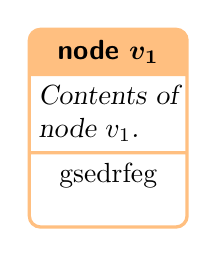
\begin{tikzpicture}
  \node[labeled node] {
    \sffamily\bfseries\boldmath
    node $v_1$
  \nodepart{two}
  \slshape
  Contents of\\
  \slshape
  node $v_1$.
  \nodepart{three}
  gsedrfeg \\
  };
\end{tikzpicture}

\end{document}